%%% Intro.tex --- 
%% 
%% Filename: Intro.tex
%% Description: 
%% Author: Ola Leifler
%% Maintainer: 
%% Created: Thu Oct 14 12:54:47 2010 (CEST)
%% Version: $Id$
%% Version: 
%% Last-Updated: Thu May 19 14:12:31 2016 (+0200)
%%           By: Ola Leifler
%%     Update #: 5
%% URL: 
%% Keywords: 
%% Compatibility: 
%% 
%%%%%%%%%%%%%%%%%%%%%%%%%%%%%%%%%%%%%%%%%%%%%%%%%%%%%%%%%%%%%%%%%%%%%%
%% 
%%% Commentary: 
%% 
%% 
%% 
%%%%%%%%%%%%%%%%%%%%%%%%%%%%%%%%%%%%%%%%%%%%%%%%%%%%%%%%%%%%%%%%%%%%%%
%% 
%%% Change log:
%% 
%% 
%% RCS $Log$
%%%%%%%%%%%%%%%%%%%%%%%%%%%%%%%%%%%%%%%%%%%%%%%%%%%%%%%%%%%%%%%%%%%%%%
%% 
%%% Code:


\chapter{Collaborative Modeling and Traceability in the Model-Based Design of CPSs}
\label{cha:traceability}


This chapter is based on the following paper:

\begin{itemize}
	
	\item  \textbf{Alachew Mengist}, Adrian Pop, Adeel Asghar, Peter Fritzson. \textbf{Traceability Support in OpenModelica Using Open Services for Lifecycle Collaboration (OSLC).} In Proceedings of the 12th International Modelica Conference, Prague, Czech Republic, May 15-17, 2017. 
	
	\item  Lena Buffoni, Adrian Pop, \textbf{Alachew Mengist}. \textbf{Traceability and impact analysis in requirement verification.} In Proceedings of the 8th International Workshop on Equation-Based Object-Oriented Modeling Languages and Tools, Munich, Germany, December 1, 2017. 
	
\end{itemize}

\section{Introduction}
\label{sec:tracaebilityintroduction}


Modeling and simulation tools have become increasingly used for industrial applications. Such tools support different 
activities in the modeling and simulation lifecycle, like specifying requirements, model creation, model simulation, \acrshort{fmu} 
export, model checking, and code generation. However, the heterogeneity and complexity of modern industrial products often require special purpose modeling and simulation tools for different phases of the development life cycle. Seamless exchange of models between different modeling tools
is needed in order to integrate all the parts of a complex product model throughout the development life cycle. 

During the past decade, the \acrshort{oslc} specifications \cite{oslc} have emerged for integrating development lifecycle tools using Linked Data \cite{linkeddatatom,linkeddata,linkeddatatim}. For traceability purposes, in particular the \acrshort{oslc} Change Management specification is relevant. In earlier work \cite{oslcelaasar} \acrshort{oslc} has successfully been demonstrated for integration of modeling tools in general, and traceability in particular. 

In \cite{debugingpop} the \acrshort{omc} supports traceability in terms of tracing generated C code back to the originating Modelica source code, but not in the \acrshort{oslc} sense, and mostly used for debugging. 

In this chapter we present new traceability support in OpenModelica where the traceability information is exchanged with other lifecycle 
tools through a standardized interface and format using \acrshort{oslc}. In particular, it supports automatic recording and tracing of
modeling activities such as creation, modification, and destruction of models, import of model description \acrshort{xml}, export of FMUs, and creation of simulation results to link models from various tools. OpenModelica supports simple queries (traces to and traces from) to present the traceability information to the user.


\section{Open Services for Lifecycle Collaboration (OSLC)}
\label{sec:tracaebilityoslc}

Open Services for Lifecycle Collaboration (OSLC) \cite{oslc} is an open-source initiative
for creating a set of specifications that enables integration of development life cycle tools (e.g.,
modeling tools, change management tools, requirements management tools, quality management
tools, configuration management tools). The goal of \acrshort{oslc} is to make it easier for tools to work together by
specifying a minimum amount of protocol without standardizing the behavior of a specific tool.

The \acrshort{oslc} specifications use the Linked Data model to enable integration at the data level via links between
tool artifacts defined as Resource Description Framework (RDF) \cite{rdffrank} resources (beside other possible representations such as
\acrshort{xml}, JavaScript Object Notation (JSON) \cite{json}, Atom, and Turtle). The resources are identified
by HTTP URIs. A common protocol to perform creation (HTTP POST) and retrieval (HTTP GET), update (HTTP PUT) and delete (HTTP DELETE) operations on resources is also specified.


\section{Traceability Design and Architecture}
\label{sec:tracaebilitydesign}


The traceability design and architecture is mainly being developed in the INTO-CPS project \cite{intocpspaper,intocps} 
which contains a set of tasks. One of these is the design of traceability and model management with the following goals \ref{intocpskenneth}:

\begin{itemize}
\item Checking the realization of requirements in models
\item Enabling collaborative work by connecting artifacts and knowledge from different users
\item Decreasing redundancy by connecting different tools to a single requirements source and allowing
a system-wide view that is not only limited to single tools
\end{itemize}

The Provenance (PROV) \cite{provluc} and \acrshort{oslc} standards presented in \cite{intocpsjohn})
are used to support traceability activities. PROV is a set of documents built on the notation and relation of
entities, activities, and agents.

The design and architecture of the traceability related tools has recently been developed in \cite{intocpskenneth} and is shown in Figure  \ref{fig:traceabilityarchitecture}. Any modeling tool written in any programming language can use these traceability standards to support the traceability of activities performed within the tool and interact with other tools.

\begin{figure}
	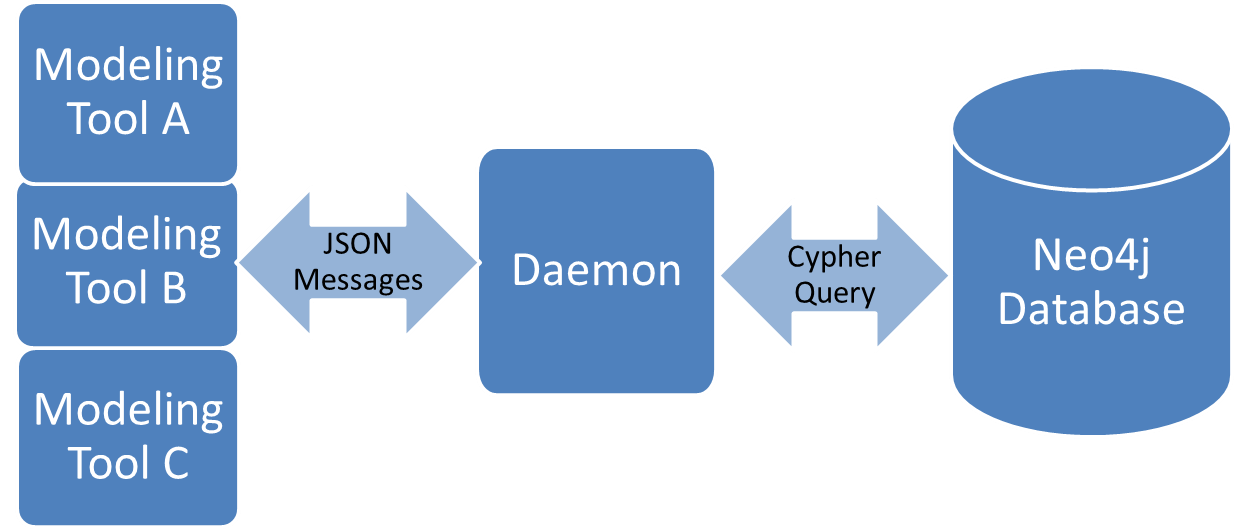
\includegraphics[width=\linewidth]{traceability_architecture.png}
	\caption{Schematic architecture of the traceability related tools.}
	\label{fig:traceabilityarchitecture}
\end{figure}


As depicted in Figure \ref{fig:traceabilityarchitecture}, the architecture is divided into three parts:

\begin{description}
\item[Modeling Tools] The modeling tools send traceability information from activities that are performed within the tools (e.g., model creation,
modification, import model description in \acrshort{xml}) to the traceability Daemon.
\item[Traceability Daemon] The traceability Daemon provides an \acrshort{oslc} interface compliant with RESTful \cite{restfulleonardo} to store the traceability 
information into the database and retrieve the traceability data from the database. It is launched and terminated by modeling tools.
\item[Neo4j Graph Database] The Neo4j database \cite{neo4j} is a graph database to store the \acrshort{oslc} triples that make up the traceability data. 

\end{description}

\section{An Example of Integrated Tools for Cyber-Physical Model Development}
\label{sec:tracaebilitytools}

OpenModelica has been successfully integrated with the INTO-CPS tool chain to trace artifacts created
during the system development process from high level requirements to simulation results. The tools involved
are Overture, 20-sim , Modelio and RTTester. The tool chain as shown in Figure \ref{fig:traceabilitytools} is defined by the connections between the system architecture and the simulation via the model description \acrshort{xml} file and the \acrshort{fmu}.

\begin{landscape}
	\begin{figure}
		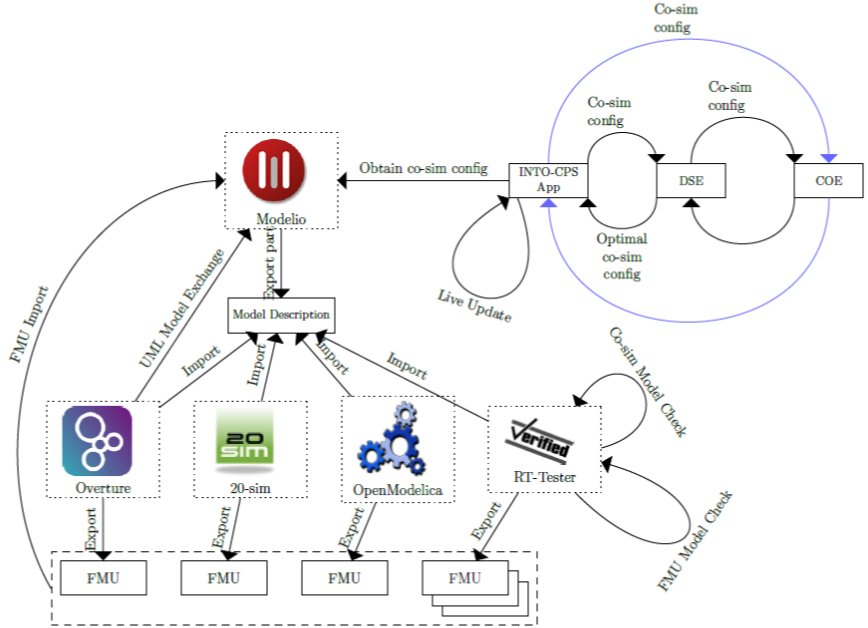
\includegraphics[width=\linewidth]{traceability_tools.png}
		\caption{An Example of integrated tools to trace artifacts created during the system development process (Bandur et al, 2016).}
		\label{fig:traceabilitytools}
	\end{figure}
\end{landscape}

The \acrshort{sysml} Connection diagram defines the components of the system and their connections. The
internals of these block instances are created in the various modeling tools and exported as FMUs. 
The modeling tools support importing the interface definition (ports) of the blocks in the Connection
diagram by importing a modelDescription.xml file containing the block name and its interface definition
linked with requirements. All tools are storing information in Git and sending information about
existing and created artifacts to the global database.

\section{Traceability and Model Management in OpenModelica}
\label{sec:tracaebilityactivities}

In the new work reported in this chapter, OpenModelica has been extended with support of traceability in the \acrshort{oslc} sense, 
where traceability information is exchanged with external tools through a standardized interface and format. The implementation is based on
an architecture and a common interface defined in \cite{intocpskenneth} for exchanging traceability information. 

The modeling activities that can be recorded automatically and traced within OpenModelica are:

\begin{itemize}
\item Model description \acrshort{xml} import (linked with requirements)
\item Model creation
\item Model modification
\item Model destruction
\item FMU export
\item Simulation result creation

\end{itemize}
The complete workflow for traceability artifacts within OpenModelica and the different components that rely on are shown in Figure \ref{fig:traceabilityworkflow}.

The following summarizes the main workflow that could be used to create and record traceability
information in OpenModelica during cyber-physical model development process.

\begin{enumerate}
\item Commit model file entity to Git repository and record the Git-hash
\item Create URIs of the activity based on the Git\-hash
\item \acrshort{oslc} triples describing the activity are generated using the URIs
\item \acrshort{oslc} triples are sent to the traceability Daemon
\item Retrieve the traceability information (traces to and traces from)

\end{enumerate}

The traceability information is represented in \acrshort{json} format. The modeling activities described by \acrshort{oslc}
triples represented in \acrshort{json} format are sent from OpenModelica to the traceability Daemon. These traces are then
sent through the traceability Daemon to the Neo4j database, where they are stored. In order to view and analyze
traceability data, this is later retrieved (traces to and traces from) from OpenModelica, through the
appropriate queries from the traceability Daemon to the database. 

\begin{figure}
	\includegraphics[width=\linewidth]{traceability_workflow.png}
	\caption{Workflow of traceability of artifacts during the system development process in OpenModelica.}
	\label{fig:traceabilityworkflow}
\end{figure}

\section{Prototype Implementation}
\label{sec:tracaebilityprototype}

We have implemented a prototype to demonstrate the idea of exchanging traceability information for
integrating lifecycle modeling tools using \acrshort{oslc}. The prototype is implemented based upon the design and
architecture presented in Section \ref{fig:traceabilityarchitecture}.

As mentioned, the implementation of this prototype is an extension of OMEdit which
is implemented in C++ using the Qt Framework graphical user interface library. For presentation reasons, we have grouped the prototype functionality into three categories: importing model description XML, model management with Git integration, and traceability support using \acrshort{oslc}, 
which are described in the following subsections.


\subsection{Import Model Description in XML}
\label{ssec:tracaebilityimprtxml}

As a preparation for the extension to support tracing for importing modelDescription.xml interface files, we 
extended OpenModelica to support importing modelDescription.xml (See Figure \ref{fig:traceabilityimportfmu}) . 

\begin{figure}
	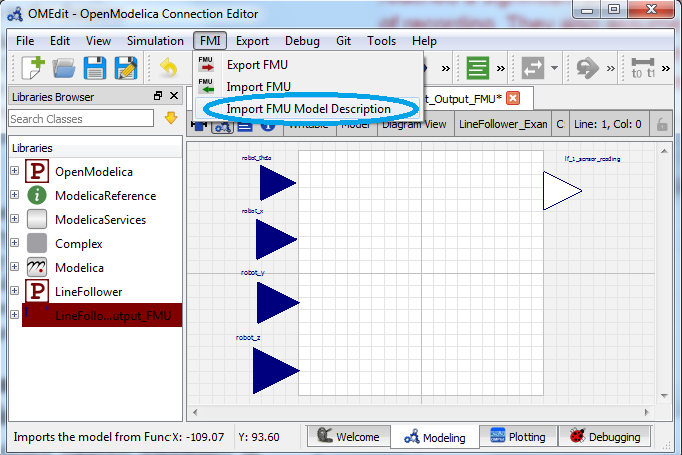
\includegraphics[width=\linewidth]{traceability_import_fmu.png}
	\caption{A screen shot of the model description XML import operation.}
	\label{fig:traceabilityimportfmu}
\end{figure}

OpenModelica can import model description \acrshort{xml} interface files (linked with requirements) created using
other system architectural modeling tools and create  Modelica models from this information. The result is a
generated file with a Modelica model stub containing the inputs and outputs specified in the model
Description.xml file. Then the user can create a complete model using the GUI via drag and drop in the
editor. Hence, the traceability chain within OpenModelica traces models linked with requirements
through model description \acrshort{xml} import, model creation, model modification, \acrshort{fmu} export and simulation results.

\subsection{Model Management with Git Integration}
\label{sec:tracaebilitygit}

One of the objectives of the traceability tooling is to manage the development process in terms of modeling
activities within the modeling tools. In order to achieve this objective access to the version control system is
required in OpenModelica. Therefore, the OpenModelica Connection Editor OMEdit has been enhanced to support Git version 
control as shown in Figure \ref{fig:traceabilitygit}.

\begin{figure}
	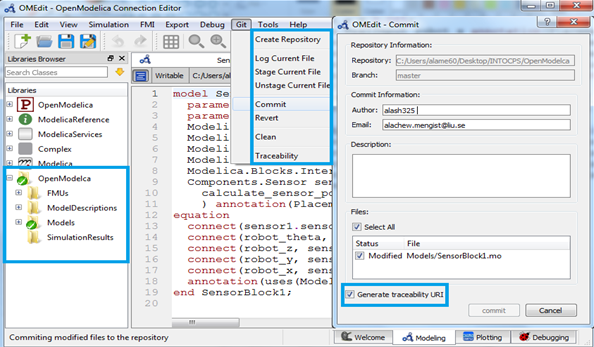
\includegraphics[width=\linewidth]{traceability_git.png}
	\caption{GUI of Git Integration in OpenModelica and functions available to create traceability URI.}
	\label{fig:traceabilitygit}
\end{figure}

The OMEdit Git integration is currently in an early stage of development but already supports some basic
functionality (See Figure \ref{fig:traceabilitygit}) such as staging modified tracing operations on files 
for commit, committing, and reverting changes. It is useful to provide viewing of status and version history 
which can be used for creating the resource URIs for the modeling activities on each new commit.

The implemented prototype also allows to create a local Git repository by selecting Git -> Create New Repository from the menu bar. 
Since the URI, as presented in \cite{intocpsjohn} is the combination of the Git-hash and the unique path for every file in the
project, creating a Git repository for traceability purposes automatically adds a structure (See the left
part of Figure \ref{fig:traceabilitygit}) for models, simulation results, FMUs, and model description \acrshort{xml} files to the Git repository.

\subsection{Traceability Support in OpenModelica}
\label{subsec:traceabilityopenmodelica}

The traceability support in OpenModelica provides a graphical user interface to interact with other lifecycle
modeling tools.

As already mentioned in Section \ref{sec:tracaebilityactivities}, OpenModelica supports traceability in the \acrshort{oslc} sense, where
traceability information is exchanged with external tools through a standardized interface and format. 
The implementation is based on the architecture and a common interface defined in \cite{intocpskenneth} for 
exchanging traceability information. OpenModelica imports the modelDescription.xml and creates a Modelica model according to the \acrshort{fmu}
interface. The generated Modelica model is completed with behavior for the \acrshort{sysml} block and the final model
is exported in the \acrshort{fmu} form. The generated \acrshort{fmu} is then used in a whole system simulation connected
according to the \acrshort{sysml} connection diagram. The \acrshort{fmu} master simulation algorithm component performs
the simulation via the INTO-CPS App. This whole chain is traced using \acrshort{oslc}.

We have designed a graphical user interface shown in Figure which allows the user to record the
traceability information and send to the traceability Daemon (\acrshort{oslc} triples in \acrshort{json} format), describing the activity
using the URIs generated in the GUI shown in Figure  \ref{fig:traceabilitygit}. The PROV and \acrshort{oslc} relations that are mainly used
in this work can be found in \cite{intocpsjohn}.

\begin{figure}
	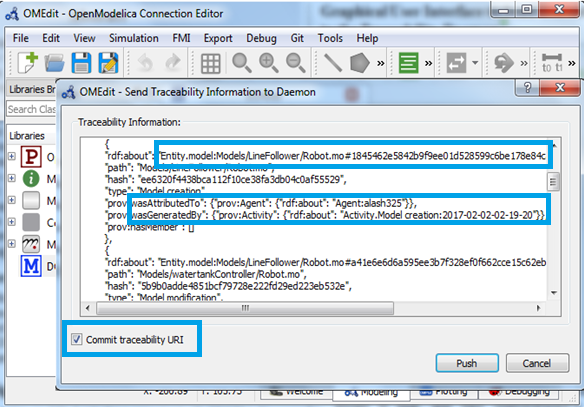
\includegraphics[width=\linewidth]{traceablity_URI_push.png}
	\caption{GUI to send traceability information to the traceability Daemon.}
	\label{fig:traceabilitypush}
\end{figure}
  
These traces are then sent through the traceability Daemon to the database via HTTP POST http://localhost:8080/
traces/push/json, where they are stored. Figure \ref{fig:traceabilitygraph} shows an example of traceability information 
sent from OpenModelica to the traceability Daemon and visualized in the Neo4j database.
\begin{landscape}
\begin{figure}
	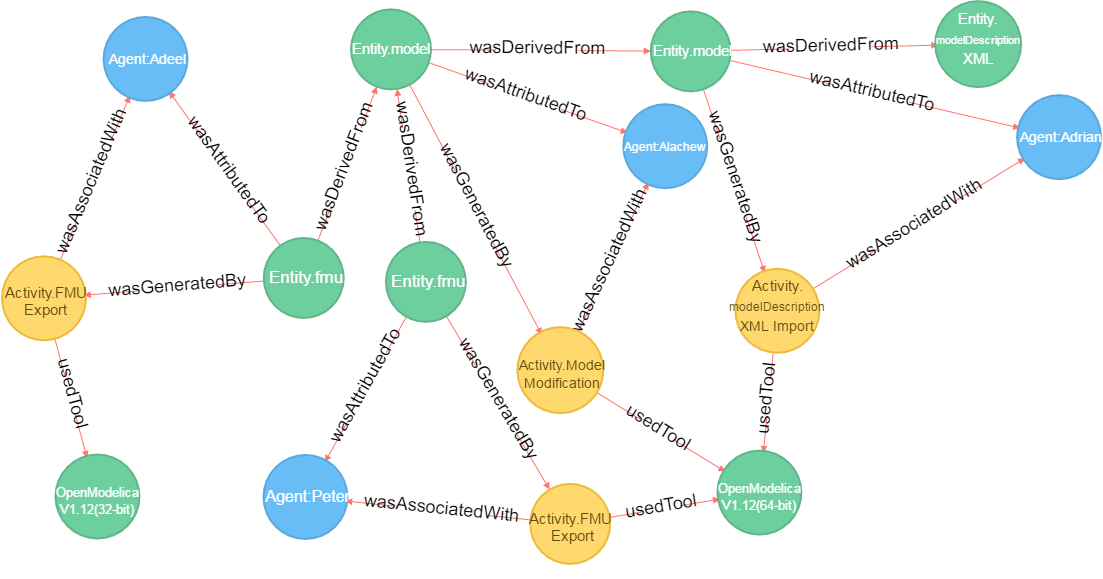
\includegraphics[width=\linewidth]{traceability_graph.png}
	\caption{An example of traceability information sent from OpenModelica to the traceability Daemon and visualized in the Neo4j database.}
	\label{fig:traceabilitygraph}
\end{figure}
\end{landscape}

Entities (e.g. Modelica files, FMUs,modelDescription XML file) are shown in green,
actions (e.g. model creation, FMU export, modelDescription XML import) are shown in yellow,
agents (e.g. users with the names {"Alachew"}, {"Adrian"}, {"Peter"}, and {"Adeel")} are shown in blue,
and their relationships "what come from what" and "what used what" (e.g. "wasGeneratedBy", "wasDerivedFrom", "usedTool") are 
shown with red arrows.

In order to view and analyze traceability data, we have also designed a graphical user interface shown in
Figure \ref{fig:traceabilityquery} which allows the user to query traceability information (traces to and traces from) from the traceability
Daemon to the database (via HTTP GET):

\begin{itemize}
\item http://localhost:8080/traces/from/<URI>/json and
\item http://localhost:8080/traces/to/<URI>/json 

\end{itemize}

\begin{figure}
	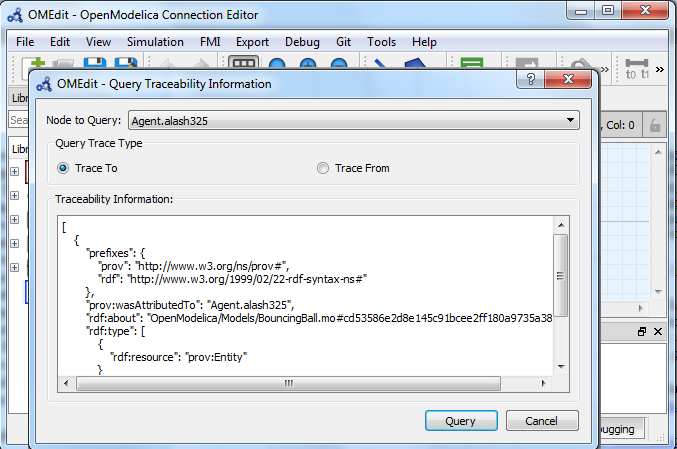
\includegraphics[width=\linewidth]{traceability_query.png}
	\caption{GUI to query traceability information from the traceability Daemon.}
	\label{fig:traceabilityquery}
\end{figure}
 
\section{Summary}
\label{sec:traceabilitysummary}

This chapter has presented a framework for traceability and model management  based on the OSLC specification standard combined with Git version control system. All operations on artifacts of interest integrated with different tools that are used in CPS design are traced. The traceability information is exchanged with external tools through a standardized interface and format. A message schema defined that ensures that all tools use the same format for sending their data,  The traceability information is stored in a graph database which can be queried for generating various reports such as impact analysis, variant handling, etc . A first prototype to query specific traceability links (traces to and traces from different entities, such as models, users, FMUs, or simulation results) from the database and display to end-users in JSON format is also presented. 

\subsection*{Acknowledgments}
\label{sec:traceabilityacknowledgments}

This work has been supported by the European Union in the H2020 INTO-CPS project. Support from
Vinnova in the ITEA3 OPENCPS project has been received. The OpenModelica development is supported
by the open-source Modelica Consortium. Special thanks to Kenneth Lausdahl, Peter Niermann, Jos H\"{o}ll,
Carl Gamble, Oliver M\"{o}ller, Etienne Brosse, Tom Bokhove, and Luis Diogo Couto for collaboration and
valuable input to traceability related tools design.


%\nocite{scigen}
%We have included Paper \ref{art:scigen}

%%%%%%%%%%%%%%%%%%%%%%%%%%%%%%%%%%%%%%%%%%%%%%%%%%%%%%%%%%%%%%%%%%%%%%
%%% Intro.tex ends here


%%% Local Variables: 
%%% mode: latex
%%% TeX-master: "demothesis"
%%% End: 
